
\section{Muhammad Abdul Gani Wijaya (1174071)}
\subsection{Teori Soal 1}
\subsubsection{Definisi Kecerdasan Buatan}
Kecerdasan buatan merupakan kecerdasan yang diterapkan pada teknologi, dan diatur serta dikembangan dalam bidang ilmiah, sebagai bentuk kecerdasan yang dibuat dari kecerdasan ilmu ilmiah yang telah ada.
\subsubsection{Sejarah Kecerdasan Buatan}
Kecerdasan buatan telah ada pada di zaman kuno dalam cerita dongeng tentang atau benda buatan yang diberkahi dengan kecerdasan atau kesadaran oleh pengrajin dan pembuatnya. Kecerdasan buatan modern menggambarkan proses cara berpikir manusia secara mekanis. Kecerdasan buatan memuncak pada penemuan komputer digital yang sudah dapat diprogram pada tahun 1940-an, sebuah mesin yang didasarkan pada perhitungan dan esensi penalaran matematika. Perangkat ini dan ide-ide nya menginspirasi para ilmuwan untuk mulai serius membahas kemungkinan membangun otak elektronik atau yang sekarang dikenal dengan kecerdasan buatan/artificial intelligence.
\subsubsection{Perkembangan Kecerdasan Buatan}
\begin{enumerate}
    \item Awal Mula Kecerdasan Buatan (1943 – 1955)
    \begin{itemize}
        \item Awal Mula AI dikerjakan oleh McCulloh dan Pitts yang membuat Neuron buatan dengan menirukan cara kerja neuron manusia dengan logika proposisional. Project tersebut bisa menyelesaikan fungsi komputasi dengan struktur neuron network.
        \item Hebbian learning, memperkenalkan aturan-aturan sederhana untuk meng-update kekuatan antar neuron.
        \item Minsky dan Edmonds berhasil membangun komputer neural network pertama pada 1950.
        \item Allan Turing dianggap sebagai orang pertama yang mengeluarkan pikiran mengenai Artificial Intelligence secara utuh pada artikelnya yang berjudul “Computing machinery and Intelligent” pada tahun 1950.
    \end{itemize}
    \item Kelahiran Kecerdasan Buatan (1956)
    \begin{itemize}
        \item McCarthy menginisiasi Dartmouth Workshop pada tahun 1956 dan melahirkan suatu bidang baru yaitu “Artificial Intelligence”.
    \end{itemize}
    \item Awal mula AI yang penuh dengan antusias dan harapan besar di masa depan (1952 – 1969)
    \begin{itemize}
        \item Sebuah tahap pengembangan aplikasi AI yang sukses jika dibandingan dengan program komputer primitif. Banyak dari aplikasi AI yang berhasil sehingga muncul istilah “evolusi mesin”
    \end{itemize}
    \item AI menjadi industry (1980 – sekarang)
    \begin{itemize}
        \item Aplikasi komersial pertama yang menggunakan sistem pakar bernama R1 yang digunakan oleh perusahaan Amerika (1982).
        \item Jepang juga membentuk proyek jangka panjang menggunakan komputer cerdas dengan berbasis Prolog.
    \end{itemize}
    \item Kecerdasan Buatan menjadi disiplin ilmu (1987 – sekarang)
    \item AI menampakkan diri di semua bidang (1995 – sekarang)
\end{enumerate}
\subsection{Teori Soal 2}
\subsubsection{Definisi Supervised Learning}
Supervised Learning adalah pembelajaran dengan diiringi oleh supervisornya. Maksud dari supervisornya adalah label pada tiap data nya. Maksud dari label adalah tag oada data yang ditambahkan dalam machine learning model. Pada contoh gambar burung di tag burung” pada setiap  masing masing image burung dan gambar ikan di tag “ikan" pada setiapvmasing masing gambar ikan. Machine learning kategori dapat berupa clasification ("ikan”, “kucing”, “burung", dsb) dan regression ( berat, tinggi dsb). Supervised learning digunakan untuk  memprediksi pola-pola dengan contoh data yang diberikan, jadi pola yang terbentuk adalah hasil pembelajaran dari data lengkap tersebut. Tentunya jika kita mengisi data baru, lalu setelah kita melakukan ETL (Extract Transform Load) maka kita akan mendapat info feature-feature dari sample baru tersebut. Kemudian dari feature-feature tersebut akan di compare dengan pattern clasification dari model yang didapat dari labeled data. Setiap label dicompare sampai selesai, dan yang memiliki percentage lebih banyak diambil sebagai prediksi akhir.
\subsubsection{Definisi Klasifikasi}
Klasifikasi adalah penggolongan atau pengelompokkan. Menurut KBBI klasifikasi adalah penyusunan bersistem dalam kelompok atau golongan menurut kaidah atau standar yang ditetapkan.  Harrolds Librarians Glossary menjelaskan bahwa klasifikasi adalah pengelompokkan benda secara logis menurut ciri-ciri kesamaannya. Lalu klasifikasi menurut Sulistyo Basuki yang menjelaskan bahwa klasifikasi merupakan proses yang digunakan untuk pengelompokkan/pengumpulan benda atau entitas yang sama, serta memisahkan benda atas entitas yang tidak sama. Namun  secara umum klasifikasi adalah suatu kegiatan yang mengelompokkan benda-benda yang memiliki beberapa ciri-ciri yang sama dan memisahkan benda yang tidak sama.
\subsubsection{Definisi Regresi}
Regresi merupakan suatu metode analisis statistik yang digunakan untuk melihat pengaruh antara dua atau lebih banyak variabel. Hubungan variabel-variabel tersebut bersifat fungsional yang diwujudkan dalam suatu model yang matematis. Analisis regresi pada variabel dibagi menjadi dua, yaitu variabel respons (response variable) atau variabel bergantung (dependent variable), dan variabel explanatory atau penduga (predictor variable) atau disebut variabel bebas (independent variable).
\subsubsection{Definisi Unsupervised Learning}
Unsupervised learning memiliki keunggulan dari unsupervised learning. Jika unsupervised learning memiliki label sebagai dasar prediksi serta membuat clasification dan regression algorithm memungkinkan. Namun pada realitanya, data real itu banyak yang tidak memiliki label. Label data akan masuk ke ERP apapun bentuk ERPnya, sedangkan jika datanya berupa natural input seperti suara, gambar, dan video tidak bisa. Pada unsupervised learning tidak menggunakan label pada saat memprediksi target feauture / variable nya. Namun menggunakan kesamaan dari attribut yang dimiliki. Jika attribut dan sifat dari data feature yang diekstrak memiliki kemiripan, maka akan dikelompokan (clustering). Sehingga nantinya akan menimbulkan kelompok kelompok (cluster). Jumlah cluster bisa tak terbatas. Dari kelompok kelompok itu model akan melabelkan, dan jika data baru yang mau di prediksi, maka akan dicocok kan dengan kelompok yang mirip featurenya.
\subsubsection{Definisi Data Set}
Dataset adalah kumpulan dari data. Yang paling umum satu
data set sesuai dengan isi tabel pada database tunggal, atau matriks data pada statistik tunggal,
di mana setiap kolom tabel mewakili suatu variabel tertentu, dan setiap baris sesuai dengan
anggota tertentu dari dataset yang dipertanyakan.
\subsubsection{Definisi Training Set}
Training Set adalah set digunakan oleh algoritma klasifikasi . Contohnya : decision tree, bayesian, neural network dll. Semuanya biasanya digunakan untuk membentuk model classifier. Menjalankan pelatihan dan diatur melalui jaringan saraf yang mengajarkan pada net cara menimbang berbagai fitur, lalu menyesuaikan koefisien berdasarkan kemungkinan mereka meminimalkan kesalahan pada hasil. Koefisien-koefisien tersebut, juga dikenal dengan parameter, akan terkandung dalam tensor dan bersama-sama mereka disebut dengan model, karena mereka mengkodekan model data yang telah mereka latih. Mereka adalah takeaways yang paling penting yang akan didapatkan dari pelatihan jaringan saraf.
\subsubsection{Definisi Testing Set}
Testing Set adalah set yang digunakan untuk mengukur sejauh mana classifier berhasil
melakukan klasifikasi dengan benar. Ini berfungsi sebagai meterai persetujuan, dan tidak menggunakannya sampai akhir. Setelah melatih dan mengoptimalkan data, dapat menguji jaringan saraf terhadap pengambilan sampel acak akhir ini. Hasil yang dihasilkannya harus memvalidasi bahwa jaring secara akurat mengenali gambar, atau mengenalinya setidaknya [x] dari jumlah tersebut. Jika tidak mendapatkan prediksi yang akurat, kembali ke set pelatihan,
lihat hyperparameter yang digunakan untuk menyetel jaringan, serta kualitas data dan lihat teknik pra-pemrosesan.

\subsection{Instalasi}
\begin{enumerate}
	\item Instalasi Library scikit dari anaconda, mencoba kompilasi dan uji coba ambil contoh kode dan lihat variabel explorer
	\hfill\break
	\begin{figure}
		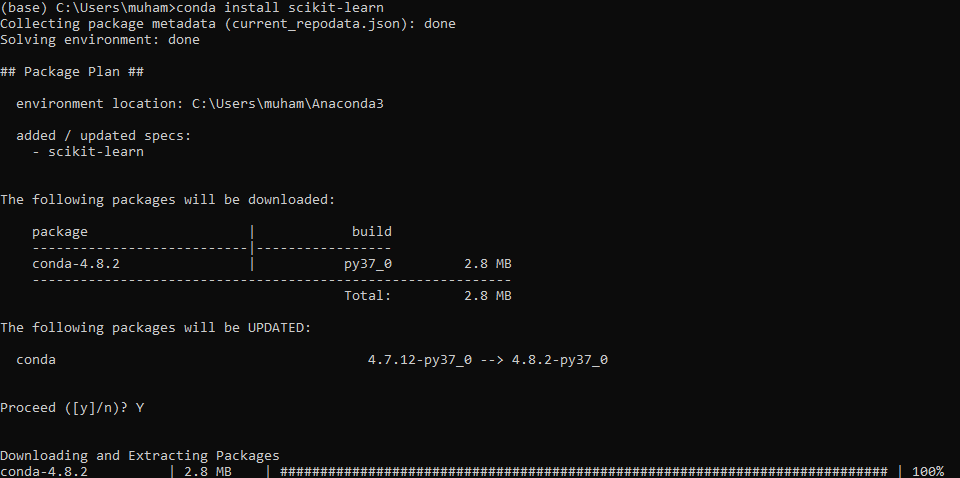
\includegraphics[width=4cm]{figures/1174071/1/1.PNG}
		\centering
		\caption{Instalasi Package Scikit}
	\end{figure}
	\begin{figure}
		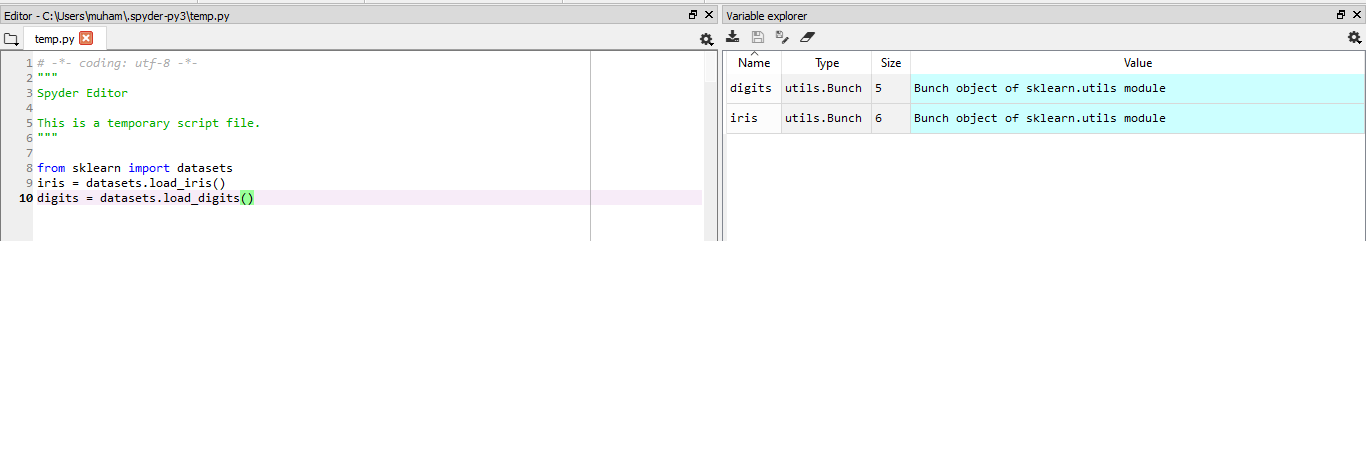
\includegraphics[width=4cm]{figures/1174071/1/2.PNG}
		\centering
		\caption{Isi Variabel Explorer Package Scikit}
	\end{figure}
	\item Mencoba Loading an example dataset, menjelaskan maksud dari tulisan tersebut dan mengartikan  per baris
	\hfill\break
	\lstinputlisting[firstline=12, lastline=20]{src/1174071/1/1174071.py}
	\item Mencoba Learning and predicting, menjelaskan maksud dari tulisan tersebut dan mengartikan perbaris
	\hfill\break
	\lstinputlisting[firstline=22, lastline=38]{src/1174071/1/1174071.py}
	\item  Mencoba Model persistence, menjelaskan maksud dari tulisan tersebut dan mengartikan per baris
	\hfill\break
	\lstinputlisting[firstline=40, lastline=59]{src/1174071/1/1174071.py}
	\item Mencoba Conventions, menjelaskan maksud dari tulisan tersebut dan mengartikan per baris
	\hfill\break
	\lstinputlisting[firstline=61, lastline=83]{src/1174071/1/1174071.py}
\end{enumerate}

\subsection{Penanganan Error}
\begin{enumerate}
	\item Screenshoot Error
	\begin{figure}
		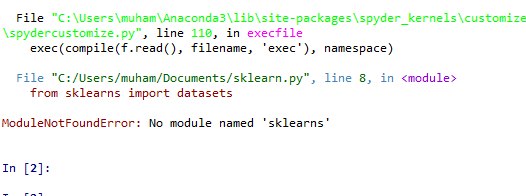
\includegraphics[width=4cm]{figures/1174071/1/error/1.PNG}
		\centering
		\caption{Import Library Error}
	\end{figure}

	\item Tuliskan Kode Error dan Jenis Error
	\begin{itemize}
		\item Import Library Error
	\end{itemize}
	\item Cara Penangan Error
	\begin{itemize}
		\item Impor Library Error
		\hfill\break
		\begin{figure}
		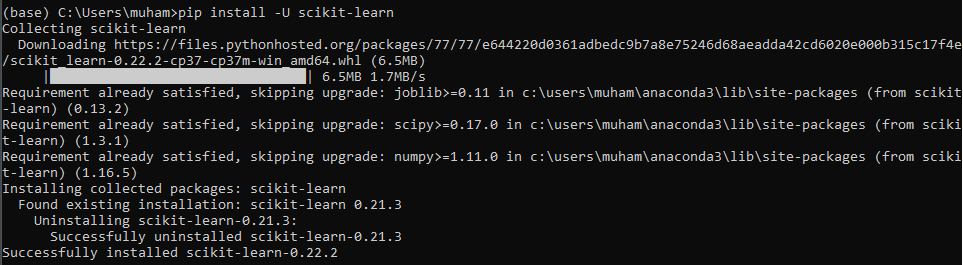
\includegraphics[width=4cm]{figures/1174071/1/error/2.PNG}
		\centering
		\caption{Install Library}
		\end{figure}
		Menginstall Library yang belum ada
	\end{itemize}
\end{enumerate}

\subsection{Bukti Tidak Plagiarisme}
\begin{figure}
	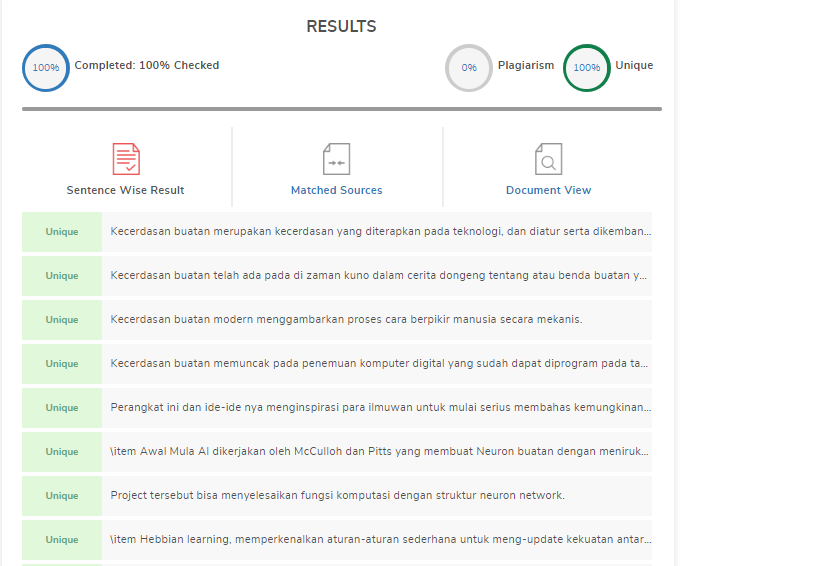
\includegraphics[width=4cm]{figures/1174071/1/plagiat/plagiat.PNG}
	\centering
	\caption{Bukti Tidak Melakukan Plagiarisme Chapter 1}
\end{figure}

\subsection{Link Youtube}
http://bit.ly/AIkem71